\subsection{Indirect Effect of Environmental Factors}
\label{sec:exp:indirect}
By observing the relation between EPI index and fragility in Figure~\ref{fig:exp:frag_relation:epi}, we find that environmental factors exhibit different kinds of influence at different stages. 
When EPI is small, the change of fragility with respect to EPI is little. When EPI is higher than a certain threshold, $E_0=50$, the changes of EPI begins to induce changes of fragility score. It could be explained, since when a state's environmental performance is too low, it tends to become too unstable such that further deterioration would have minor effect.  

Therefore, we establish different models for states which are below and higher than the threshold, respectively, to explain the indirect effect of environmental factors in terms of moderator and mediator effects formulated in Section~\ref{sec:model:indirect}.

\subsubsection{When the Index $\rm{EPI} > 50$}
These states are comparably environmentally stable. For these states, change of environment significantly influence fragility. The relationship is illustrated in Figure~\ref{fig:exp:indirect:case2}.
\begin{figure}[tbp]
    \centering
   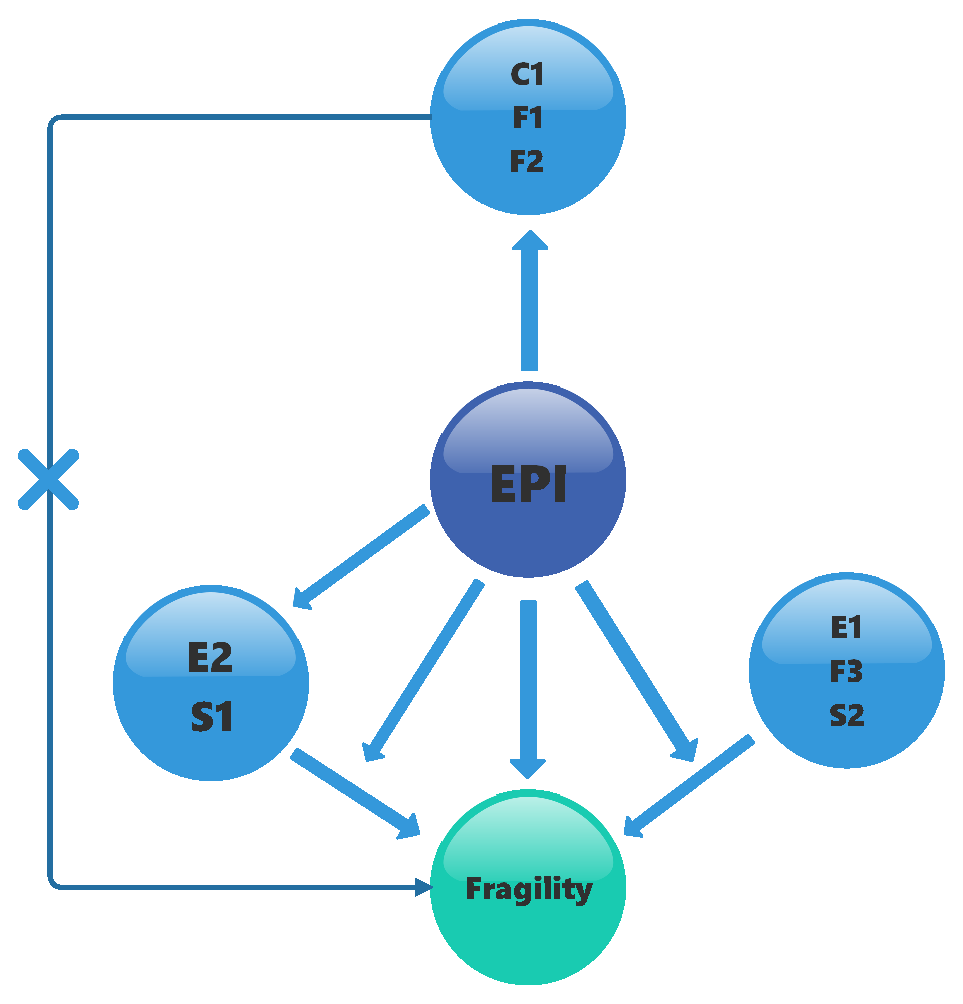
\includegraphics[width=.4\linewidth]{figs/larger50.eps} 
   \caption{Illustration of Effects of Environmental Performance when EPI $> 50$}
   \label{fig:exp:indirect:case2}
\end{figure}

\vpara{Moderator Effect}
To examine the moderator effect, we establish a linear regression model:
\begin{equation}
    \FFS \sim \rm{EPI} + F \times\rm{EPI}+ F
    \label{eqn:indirect:moderator:reg} 
\end{equation}
where
\begin{equation}
   S= \sum\rm{E}_k + \sum\rm{P}_k + \sum\rm{S}_k + \sum\rm{C}_k + \sum\rm{X}_k
\end{equation}
is the sum of economic, political, social, cohesion indicators, and external indicators used in FSI index, as in Table~\cite{FSI_index}. 
The second term is the effect of moderators. 

We select significant variables from the regression model in Eqn.~\ref{eqn:indirect:moderator:reg} by bidirectional step regression. The selected variables, their coefficients, p-value and level of significance are listed in Table~\ref{tab:exp:indirect:moderator:case1}.

\begin{table}[htbp]
    \small
    \centering
   \begin{tabular}{|l|ccc|}\hline
      Var. & Coef. & P-val. & Level \\ \hline
      EPI & 0.050534 & 7.44e-11 & Super \\ \hline
      E1 & 0.337434 & 0.003849 & High \\ \hline
      E2 & -0.404308 & 0.002120 & High \\ \hline
      P3 & 0.363195 & 0.009289 & High \\ \hline
      EPI$\times$E1 & -0.004889 & 0.006607 & High \\ \hline
      EPI$\times$E2 & 0.006458 & 0.002109 & High \\ \hline
      EPI$\times$P3 & -0.005600 & 0.011503 & Medium \\ \hline
      EPI$\times$S2 & -0.004610 & 0.000142 & High \\ \hline
   \end{tabular} 
   \caption{Moderator Effect when $\EFF > 50$}
   \label{tab:exp:indirect:moderator:case1}
\end{table}

We see that E1, E2, P3 appears both individually in Table~\ref{tab:exp:indirect:moderator:case1} and also as factors of cross products. Therefore, EPI moderates the relations between these variables and fragility. There is no other variable that appear individually; therefore, we are confident that EPI act as a moderator between human factors and fragility.

To conclude,
EPI moderates the relation of these following human factors:
\begin{itemize}
    \item Economic Decline
    \item Uneven Economic Development
    \item Human Rights and Rule of Law
    \item Refugees and IDPs 
\end{itemize}
Indeed, environmental performance does not have a clear and direct relationship with these variables. The moderator effect of environment on many economic indicators can be explained by Kuznets curve~\cite{kuznets1955economic,kuznets1966modern}.


\vpara{Mediator Effect}
EPI's direct impact on fragility is already verified in Table~\ref{tab:exp:direct} and Table~\ref{tab:exp:indirect:moderator:case1}, since predicting fragility using EPI alone would result in a even higher level of significance as in the model of Table~\ref{tab:exp:indirect:moderator:case1}.

We verify the role of human factors by establishing regression models in which EPI is used to predict each individual indicator of FSI. When EPI significantly predicts an indicator, we establish another regression model, in which EPI and the indicator jointly predict fragility. 

These following indicators are mediator variables, through which environmental factors indirectly exhibit influence on fragility:
\begin{itemize}
   \item Public Services
   \item Demographic Pressures
\end{itemize}
Clearly, environmental factors directly influences a state's public services and demographic pressures. The influence then propagates to fragility.

\subsubsection{When the Index $\rm{EPI} < 50$}
These states are environmentally fragile, and fragility of these states is no longer sensitive to environmental fragility.

\vpara{Mediator Effect.}
We establish a regression model, using EPI to predict fragility, for states with EPI$<50$. 
However, the coefficient of EPI in this case is $ -0.0003162 $, with p-value being 0.225. EPI is insignificant, which is also verified in Figure~\ref{fig:exp:frag_relation:epi}. Since environment does not influence fragility directly, mediator effect is impossible.

\begin{table}[htbp]
\centering        
\small
   \begin{tabular}{|l|ccc|}\hline
    Var. & Coef. & P-val. & Level \\ \hline
      C1 & 6.174e-4 & 0.033153 & Medium \\ \hline
      C2 & -1.334e-3 & 0.001708 & High \\ \hline
      C3 & 6.624e-3 & 0.001896 & High \\ \hline
      E1 & 9.62e-3 & 0.004577 & High \\ \hline
      E3 & -4.759e-3 & 1.63e-14 & Super \\ \hline
      P1 & 8.484e-3 & 0.006177 & High \\ \hline
      P3 & -1.391e-2 & 0.000802 & High \\ \hline
      S2 & 2.320e-3 & 5.95e-8 & Super \\ \hline
      X1 & 7.863e-4 & 0.005399 & High \\ \hline
      EPI$\times$C3 & -1.68e-4 & 0.000992 & Medium \\ \hline
      EPI$\times$P3 & 3.123e-4 & 0.000822 & Medium \\ \hline
   \end{tabular}
   \caption{Moderator Effect when EPI$<50$}
   \label{tab:exp:indirect:moderator:case2}
\end{table}

\vpara{Moderator Effect.} The result of moderator effect when EPI$<50$ is in Table~\ref{tab:exp:indirect:moderator:case2}.

Although the state is fragile, and its fragility is insensitive to environmental change, environments moderates the impact of two human factors, C3 and P3, as clearly demonstrated in the table. C3 and P3 are respectively Group Grievance and Human Rights and Rule of Law.

\subsection{Case Study}
\vpara{A Fragile State: Iraq.} 
Iraq is, by FSI, one of the 10 most fragile states in the world. 
Also, the EPI Index of Iraq is below 50, the tipping point for environment performance. 
Using regression model in Eqn.~\ref{eqn:indirect:moderator:reg} and coefficients in Table~\ref{tab:exp:indirect:moderator:case2}, we calculate the fragility score of Iraq to be 0.962, while the fragility score of Iraq calculated in Section~\ref{sec:exp:frag} is 0.9615. The low residual verifies the efficiency of our model for environmentally fragile states.

Utilizing PSM, we find that the direct impact of environmental fragility on FSI score of Iraq is -0.075.

By taking partial derivative, we obtain
$$
\frac{\partial{s_f}}{\partial{\rm{EPI}}} = -1.68 \times 10^{-4} \rm{C3} + 3.123 \times 10^{-4}\rm{P3}
$$
Where C3 is for Group Grievance, and P3 is for Human Rights and Rule of Law. 
Plugging in the values of corresponding indicators, we obtain that  
$$
\frac{\partial{s_f}}{\partial{\rm{EPI}}} = -1.6128\times 10^{-3} +2.7170 \times 10^{-3} = 0.0075 $$

Combining direct and indirect effect, we see that decreasing EPI leads to increase in fragility of Iraq. Bad environment leads to more fragile state.

We may further investigate the moderator effect of EPI. If we see EPI as a constant, the coefficient of C3 can be seen as $-1.68e-4\rm{EPI}+6.624e-3$, and the coefficient of P3 is $3.123e-4\rm{EPI} - 1.391e-2 $. That is to say, decreasing EPI would amplify the effect of Group Grievance and Human Rights and Rule of Law. 

To explain, Group Grievance focuses on divisions and schisms between different groups in society, and is incluced by inequal distribution of resources, divisions, and communal violence.
Since further deterioration of environmental performance in a fragile state would deplete resources, such effect is expectable. This also creates human rights issues, since bad environment in this case could even harm people's basic right of living. 

\vpara{A Stable State: Mauritius}
Mauritius is a country whose EPI is larger than the threshold 50, and is not in the list of top ten vulnerable in terms of FSI index. The fragility score is $0.315$, confirming that it is comparably stable.

The direct effect calculated by PSM is -0.047. As we analyzed, environmental performance's indirect effect is exhibited both as a moderator variable and a mediator variable. 

By similar analysis in the last part, we find that better environmental performance alleviates the pressures of human rights (P3), uneven economic development (E2), and economic decline(E1). 

Unlike for environmentally fragile states, the moderator effect takes place. For Mauritius, increase of environmental performance would improve its public services and alleviate its demographic pressures.


\hide{
观察EPI和国家脆弱的曲线我们可以很明显的看到EPI对于国家脆弱的影响是分阶段的——在EPI较小的时候,国家脆弱随着EPI变化发生变动较小,但是随着EPI的增大,当EPI到达经过某一点后,EPI的变化开始导致国家脆弱发生显著的变化,关于这个转折点,我们在后面的模型中也会提及他的含义。这样的原因是因为当环境变差到一定程度后,国家已经处于崩溃的边缘了,这个时候环境的继续恶化将不再显著影响国家的脆弱程度,因此为了使得结果更加符合事实,我们对转折点之前的国家和转折点之后的国家分别建模使得模型更加符合实际的情况。并且对于这两类国家都分析环境因素在其中起到的间接影响的作用。

\subsection{EPI>转折点的情况}
这类国家是环境相对不太差的情况,对于这类国家,环境的变化还是能比较显著的影响国家脆弱的,下面分成调节效应和中介效应来分析对于这些国家环境因素起到的间接影响:
\subsubsection{调节效应}
所谓的调节作用就是说调节因素影响了自变量X对因变量,在这个问题中,人为因素看起来是对国家崩溃影响更加直接的因素,要分析环境因素的调节作用,就要看环境因素是否影响了认为因素和国家脆弱之间的关系,为了验证这种关系,我们首先建立FSI的各项指标对国家脆弱的线性回归模型:
$$Fragility = \beta_0 + \beta_1C_1 + \beta_2C_2 + \beta_3C_3 + \beta_4E_1 + \beta_5E_2 + \beta_6E_3 + \beta_7F_1 + \beta_8F_2 + \beta_9F_3 + \beta_{10}S_1 + \beta_{11}S_2 + \beta_{12}X_1$$

为了体现EPI的调节作用,我们在模型中加入EPI和EPI与FSI各项指标的乘积作为交叉项,加入上述的回归模型中,验证交叉项的系数的显著性,我们得到下面的回归方程:
$$Fragile = -3.56144+0.050534EPI+0.337434E_1-0.404308E_2+0.363195F_3+0.062685S_1+0.322859S_2-0.04889EPI \times E_1 + 0.006458 EPI \times E_2 - 0.005600 EPI \times F_3 - 0.004610 EPI \times S_2$$
从上述的回归表达式我们可以看到,所有出现交叉项的FSI的元素都单独出现在回归方程中,这就说明EPI对这些交叉项的因素的影响是调节效应,具体来说EPI对$E_1,E_2,F_3,S_2$产生了调节效应,不但这四个因素出现在了回归方程中,他们和EPI的乘积也出现在了回归方程中,但是我们要注意到的是,回归方程中除了这些因素还出现了其他因素,这就是说并不是所有的因素都是受到EPI的影响的,有一些人为因素和环境因素的相关性较低,因此环境因素对他们和国家脆弱之间的影响不显著。这在模型中也是合理的。

\subsubsection{中介效应}
中介效应是说自变量X对自变量Y的影响是通过中介变量M进行传递的,中介效应主要分成三个部分
\begin{itemize}
    \item[1.] 自变量X对因变量Y的回归系数显著
    \item[2.] 自变量X对中介变量M的回归系数显著
    \item[3.] 在加入中介变量M后自变量X对因变量Y的参数显著性明显下降,中介变量M对因变量Y的回归系数显著
\end{itemize}
在我们的模型中,要验证环境对国家脆弱的中介影响,环境因素为自变量X,国家脆弱是因变量Y,人为因素是中介变量M,环境因素对国家脆弱的回归系数显著,环境变量对国家脆弱的回归系数显著,在加入人为因素后,环境因素对国家脆弱显著性明显下降,人为因素对国家脆弱回归系数显著。

下面验证环境通过中介变量人为因素对国家脆弱的中介因素:
分别对FSI的12个因素中的每一个和EPI共同对国家脆弱做线性回归,观察回归得到的参数的显著性,符合因素的参数显著而EPI的参数不显著的因素共有$C_1,E_2,F_1,F_2,F_3,S_1$这六个因素,再对这六个因素和EPI之间的关系的显著性进行检验,得到的结果是EPI对这六个因素的回归系数都显著,结合上一部分得到的调节变量的结果,$E_2,F_3$也出现在了调节效应的方程中,这说明只有这两个因素受到了环境的作用并且将环境的作用传递到了国家脆弱指标中,剩余的几个因素虽然也受到了环境的中介作用,但是综合所有变量后影响并不显著。

综合上面提到的中介效应和调节效应我们对环境相对较好的国家的环境因素产生的影响进行分析:
环境对国家脆弱的影响分成两种形式——调节效应和中介效应。其中调节效应是环境因素在自变量影响国家脆弱的过程中产生了影响,这些自变量分别为经济衰减、不平衡经济发展、人权、难民,环境在这些因素影响国家脆弱的过程中扮演的角色不那么容易被理解,因为看起来环境和这些因素并没有很显著的直接相关性,但是事实上这正是调节效应的特点,因为环境不是直接作为自变量参与因变量的影响,而是通过交叉项影响因变量,因此环境和这几个因素的关系不是那么的明显,但是根据环境库兹涅茨曲线,环境是会对经济产生影响的(Kuznets, 1955),他们之间存在倒U形的关系,因此环境是会对经济衰减和不平衡经济发展产生影响的。类似的,环境对人权和难民的影响也是隐性的而不是直接影响这些因素,因此可以通过调节效应作出解释。另一方面,环境还能通过公共服务和人口压力对国家脆弱产生中介效应,这两个因素和环境情况有着显著的关系,比如当环境较差的时候,人口压力显然会更大,因此环境会通过他们对国家脆弱产生影响。


\subsection{EPI<转折点的情况}
这类国家是环境比较差的国家,对于这些国家通常国家脆弱程度已经比较大了,环境的恶化只能导致国家脆弱缓慢增长。下面我们将间接影响分成调节作用和中介效应两类分别分析:
\subsubsection{中介效应}
在验证中介效应的时候,首先对EPI和国家脆弱作线性回归,这个时候我们会发现,EPI的系数并不显著,这是可以从EPI和国家脆弱的关系图中看到的——当EPI减小到一定程度的时候国家脆弱指标改变的幅度也很小,即便EPI的变化十分的显著,此时国家的环境继续恶化对国家的崩溃已经没有显著的影响了,因此对于这样的国家EPI并不会通过中介效应对国家脆弱产生影响。
\subsubsection{调节效应}
在上面的分析中我们看到对于环境情况较差的国家来说,环境并不会通过中介效应对国建脆弱产生影响,但这并不意味着环境就对国家脆弱没有影响,事实上我们可以想到的是,国家的环境的好坏可能会改变人为因素对于国家脆弱的影响,即便现在的环境已经很糟糕了,虽然环境本身的改变不会改变国家脆弱,但是会影响其他因素对国家脆弱的影响,这也就是环境因素的调节作用,下面我们来验证环境因素的调节效应——在模型中加入EPI和EPI与FSI各项指标的乘积作为交叉项,加入上述的回归模型中,验证交叉项的系数的显著性,我们得到下面的回归方程:
$$Fragile = 9.399 \times 10^{-1} + 6.17 \times 10^{-4} C_1 -1.33 \times 10^{-3} C_2 +6.62 \times 10^{-3}C_3+9.62 \times 10^{-3}E_1 -4.759 \times 10^{-3}E_3 +8.484 \times 10^{-3} F_1 -1.391 \times 10^{-2} F_3+2.320 \times 10^{-3} S_2 +7.863 \times 10^{-4} X_1 -1.68 \times 10^{-4} EPI \times C_3 +3.123\times 10^{-4} EPI\times F_3$$
观察上面的回归方程我们可以看到回归方程中出现的交叉项有$EPI\times C_3,EPI\times F_3$,这两个因素的含义分别是集体诉讼和人权,也是和环境看起来没有直接因果关系的因素,因此环境在其中扮演的作用是环境影响了这两个因素对国家脆弱的影响,因为这些因素会显著的影响国家的脆弱,环境因素起到的作用是在不同的环境条件下,这些因素对国家脆弱的影响会出现不同。

综合上面两个部分,对于环境较差的国家,环境对于国家脆弱的间接影响只体现在调节效应中,因为此时环境继续恶化本身不会直接改变国家的脆弱情况,但是一些因素对国家脆弱的影响在不同的环境条件下回出现不同,因此环境条件会通过这样的调节作用间接影响国家脆弱。所以在没有中介效应的情况下,我们不需要对中介因素再做检验,上述的调节效应的模型就是这些国家的最终模型。

\section{Task2}
这一部分我们针对一个FSI排名较差的国家来具体说明上述模型的有效性,我们先选择环境指标EPI在转折点以下的Iraq,通过将Iraq的各个指标带入我们的模型中可以得到Iraq的Fragility为0.9632,而我们得到的Iraq的真实的Fragility为0.9615,两者基本吻合,这就说明了我们的模型对于环境较差的国家是有较好的表现的。下面我们来详细表示气候变化是如何影响伊朗这个国家的脆弱性的。在上面的分析中我们已经看到,对于伊朗这样的环境较差的国家,环境对于国家脆弱的影响主要通过调节效应的作用,调节作用体现在回归方程的交叉项中,我们通过求偏导就可以得到环境改变对国家脆弱的影响:
$$\frac{\partial{Fragile}}{\partial{EPI}} = -1.68 \times 10^{-4} C_3 + 3.123 \times 10^{-4}F_3$$
因为我们现在已经有了伊朗的各项指标,所以我们将伊朗的具体指标带入上式得到:
$$\frac{\partial{Fragile}}{\partial{EPI}} = -1.6128\times 10^{-3} +2.7170 \times 10^{-3}$$
因此我们可以计算得到现在的状态下偏导数是0.0075,为正值。但是在间接影响到的同时,环境因素还对国家的脆弱程度存在着直接的影响,通过前面的模型中叙述的PSM方法,我们可以计算得到当EPI为43.2的时候,环境对于国家脆弱的影响为-0.075,综合直接影响和间接影响我们就可以得到此时环境变差仍然能导致国家脆弱的上升,相反如果没有这样的环境恶化,也就是环境指标上升,国家脆弱就会相应的下降,此时国家就不会像现在一样脆弱,综上就是对于一个FSI排名靠后的国家的环境对于国家脆弱的影响。

\section{Task3}
在上一部分的模型验证中我们选择了环境指标低于转折点的国家,这一部分我们选择FSI不在倒数十个国家中的国家——毛里求斯,通过之前建立的模型得到国家脆弱指数为0.315,因此毛里求斯属于较为稳定的国家。
因为对于环境指标大于转折点的国家来说,间接影响分成了调节效应和中介效应,而中介效应是能够统一在调节效应中的,因此我们直接通过调节效应的模型来分析环境对国家脆弱的影响,类似上面的做法,我们对EPI求偏导:
$$\frac{\partial{Fragile}}{\partial{EPI}} = 0.0050534 - 0.004889E_1 +0.006458E_2 - 0.0056F_3 - 0.00461S_2$$
下面带入毛里求斯的实际指标,计算得到偏导数为0.022,同样的,在这个模型的分析中我们也需要通过PSM分析环境对国家脆弱的直接影响,带入毛里求斯的EPI计算得到直接影响为-0.047,综合直接和间接影响两项指标,我们可以得到环境对国家脆弱的总影响为-0.025,这是符合预期的。


}